%!TEX root = ../main.tex
%%%%%%%%%%%%%%%%%%%%%%%%%%%%%%%%%%
% Links:
%
% Difficulty:
% Companies: 
%%%%%%%%%%%%%%%%%%%%%%%%%%%%%%%%%%


%\begin{figure}
%	\centering
%	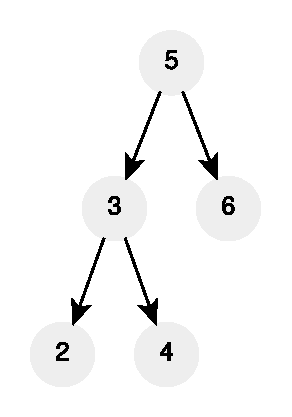
\includegraphics[width=\textwidth]{sources/merge_k_sorted_lists/images/example1}
%	\caption[Sample short cpation]{Sample Caption}.
%	\label{fig:merge_k_sorted_lists:example1}
%\end{figure}

\chapter{Merge $k$ sorted lists}
\label{ch:merge_k_sorted_lists}
\section*{Introduction}
The problem discusses in this chapter is quite interesting because it is heavily influenced and based on the familiar  merge-sort algorithm\cite{wiki:mergesort} which is a divide and conquer algorithm that works by first splitting a list into smaller and smaller ones (see figure \ref{fig:merge_k_sorted_lists:example_mergesort}) and then sorts them separately and then it merges them a pair at the time preserving the sorting property (see figure \ref{fig:merge_k_sorted_lists:example_mergesort_1}). 
The merge phase is what we are going to focus in this chapter and in particular we will extend it so that we can merge more than a pair of sorted lists together at the same time. 

Coming up with a brute-force solution for merging $k$ lists together is not hard but the end solution is rather inefficient. A faster and more efficient solution requires a bit more effort, but luckly there are quite a number of different approaches that we can take to get to one of them. In the remaining of the chapter we will have a look at the brute-force solution (in Section \ref{merge_k_sorted_lists:sec:bruteforce}) and then we will look at two approaches we can take to lower the overall time and space complexity (in Section \ref{merge_k_sorted_lists:sec:priorityqueue} and \ref{merge_k_sorted_lists:sec:divideetimpera}).


\begin{figure}
	\centering
	\begin{subfigure}[t]{0.80\textwidth}
		\caption[]{First phase of the merge-sort where the a list is recursively split into smaller ones (~ half the original length) until we are left with lists of size $1$}.
		\label{fig:merge_k_sorted_lists:example_mergesort}
		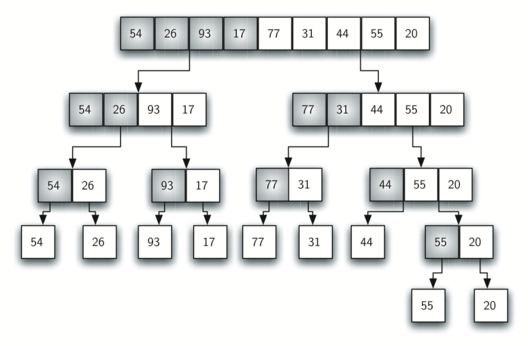
\includegraphics[width=\textwidth]{sources/merge_k_sorted_lists/images/mergesort_example}
	 \end{subfigure}
	\hfill
	\begin{subfigure}[t]{0.80\textwidth}
		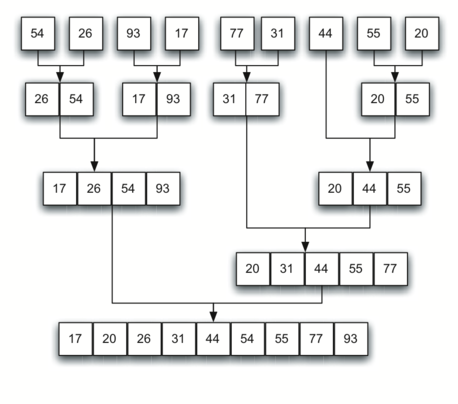
\includegraphics[width=\textwidth]{sources/merge_k_sorted_lists/images/mergesort_example_1}
		\caption[]{Second phase of the merge-sort where the split lists are recursively merged preserving the sorting property.}.
		\label{fig:merge_k_sorted_lists:example_mergesort_1}
	 \end{subfigure}
\end{figure}

\section{Problem statement}
\begin{exercise}
\label{example:merge_k_sorted_lists:exercice1}
Write a function that, given $k$ lists that are sorted in ascending order, merges them into a new sorted list.

	%example1
	\begin{example}
		\label{example:merge_k_sorted_lists:example1}
		\hfill \\ 
		Given \inline{L=[[1,4,5],[1,3,4],[2,6]} the function returns \inline{[1,1,2,3,4,4,5,6]}
	\end{example}

	%example2
	\begin{example}
		\label{example:merge_k_sorted_lists:example2}
		\hfill \\ Given \inline{L=[[1,2,3],[4,5,6],[7,8,9]} the function returns \inline{[1,2,3,4,5,6,7,8,9]}
	\end{example}

	\begin{example}
		\hfill \\ Given \inline{L=[[7,8,9],[4,5,6],[1,2,3]} the function returns \inline{[1,2,3,4,5,6,7,8,9]}
	
	\label{ex:merge_k_sorted_lists:example3}
	\end{example}

\end{exercise}

\section{Clarification Questions}

\begin{QandA}
	\item 
	\begin{answered}
		\textit{}
	\end{answered}
	
\end{QandA}

\section{Discussion}
\label{merge_k_sorted_lists:sec:discussion}


\subsection{Brute-force}
\label{merge_k_sorted_lists:sec:bruteforce}

\begin{minipage}{\linewidth}
	\lstinputlisting[language=c++, caption={Sample Caption},label=list:merge_k_sorted_lists]{sources/merge_k_sorted_lists/merge_k_sorted_lists_solution1.cpp}
\end{minipage}


\subsection{Priority-queue approach}
\label{merge_k_sorted_lists:sec:priorityqueue}

\subsection{Divide et impera}
\label{merge_k_sorted_lists:sec:divideetimpera}

